\documentclass[tikz,border=5mm]{standalone}
\usetikzlibrary{angles,quotes,calc}

\begin{document}
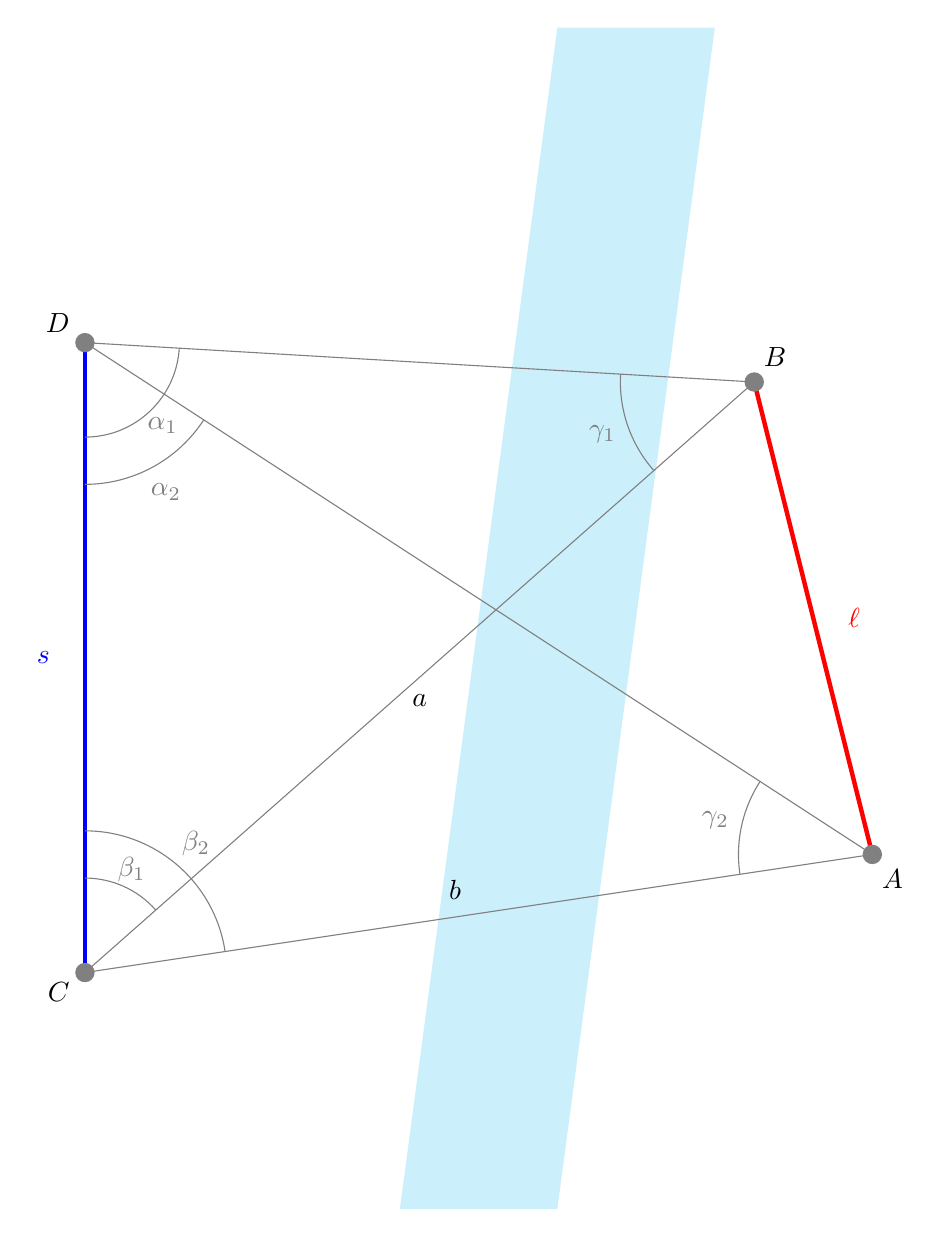
\begin{tikzpicture}
  % coordinates of the vertices
  \coordinate (C) at (0, 0);
  \coordinate (A) at (10, 1.5);
  \coordinate (D) at (0, 8);
  \coordinate (B) at (8.5, 7.5);

  % define coordinates for the cyan band
  % A diagonal band crossing the figure
  \coordinate (BandTopRight) at (8, 12);
  \coordinate (BandTopLeft) at (6, 12);
  \coordinate (BandBottomRight) at (6, -3);
  \coordinate (BandBottomLeft) at (4, -3);

  % The background cyan band, made somewhat wider to cover more
  \fill[cyan!20] (BandBottomLeft) -- (BandBottomRight) -- (BandTopRight) -- (BandTopLeft) -- cycle;

  % Thick, colored lines
  \draw[ultra thick, blue] (C) -- (D) node[midway, left=3mm, blue] {$s$};
  \draw[ultra thick, red] (A) -- (B) node[midway, right=3mm, red] {$\ell$};

  % Thin, gray lines
  \draw[thin, gray] (A) -- (D);
  \draw[thin, gray] (B) -- (C);
  \draw[thin, gray] (A) -- (C);
  \draw[thin, gray] (B) -- (D);

  % Side labels
  \node[black] at ($(B)!0.5!(C)+(0,-0.3)$) {$a$};
  \node[black] at ($(A)!0.5!(C)+(-0.3,0.3)$) {$b$};

  % Points (filled circles and labels)
  \fill[gray] (A) circle (3.5pt) node[anchor=north west, black, yshift=-2pt] {$A$};
  \fill[gray] (B) circle (3.5pt) node[anchor=south west, black, yshift=2pt] {$B$};
  \fill[gray] (C) circle (3.5pt) node[anchor=north east, black, xshift=-2pt] {$C$};
  \fill[gray] (D) circle (3.5pt) node[anchor=south east, black, xshift=-2pt] {$D$};

  % Angles and their labels
  
  % Corner D
  \pic[draw, thin, gray, "$\alpha_1$", angle radius=1.2cm, angle eccentricity=1.2] {angle = C--D--B};
  \pic[draw, thin, gray, "$\alpha_2$", angle radius=1.8cm, angle eccentricity=1.2] {angle = C--D--A};

  % Corner B
  \pic[draw, thin, gray, "$\gamma_1$", angle radius=1.7cm, angle eccentricity=1.2] {angle = D--B--C};

  % Corner C
  \pic[draw, thin, gray, "$\beta_1$", angle radius=1.2cm, angle eccentricity=1.2] {angle = B--C--D};
  \pic[draw, thin, gray, "$\beta_2$", angle radius=1.8cm, angle eccentricity=1.2] {angle = A--C--D};

  % Corner A
  \pic[draw, thin, gray, "$\gamma_2$", angle radius=1.7cm, angle eccentricity=1.2] {angle = D--A--C};

\end{tikzpicture}
\end{document}